% The hyp_to_gds.py input/output contract: what the converter reads, the order
% of the stages it runs, and every file it writes.
\documentclass[border=4pt]{standalone}
\usepackage{tikz}
\usetikzlibrary{arrows.meta, positioning, calc}
\usepackage[T1]{fontenc}
\usepackage{lmodern}

\definecolor{IHPfg}{RGB}{0,80,139}
\definecolor{IHPaccent}{RGB}{109,112,114}
\definecolor{IHPlight}{RGB}{225,238,250}
\definecolor{IHPgreen}{RGB}{65,155,75}
\definecolor{IHPgreylight}{RGB}{242,242,243}

\begin{document}
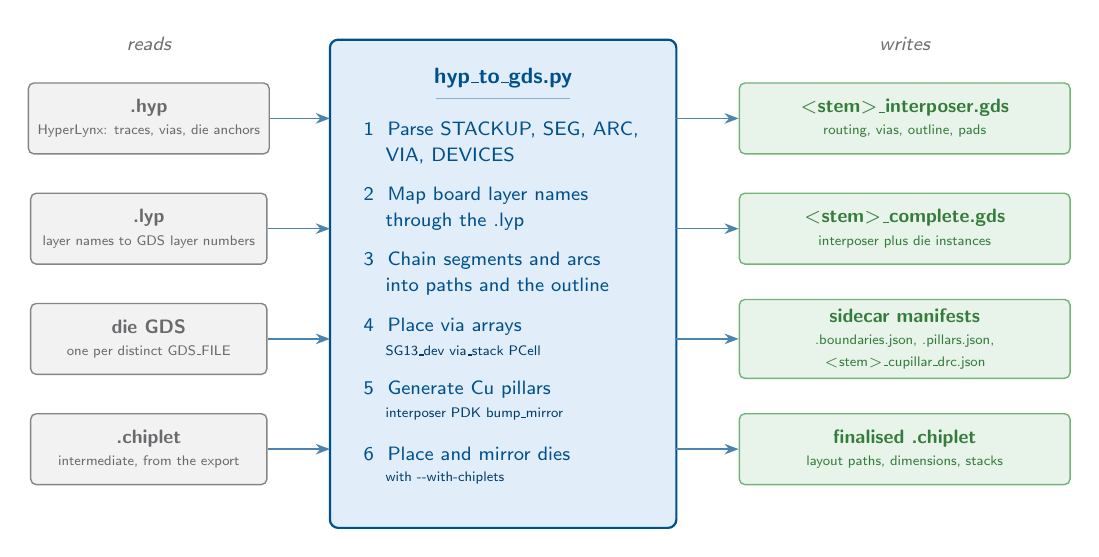
\begin{tikzpicture}[
    >=Stealth,
    infile/.style={
        rectangle, rounded corners=2pt,
        draw=IHPaccent!85, fill=IHPgreylight, line width=0.5pt,
        minimum width=30mm, minimum height=9mm,
        font=\sffamily\scriptsize, text=IHPaccent!95!black, align=center
    },
    outfile/.style={
        rectangle, rounded corners=2pt,
        draw=IHPgreen!75, fill=IHPgreen!12, line width=0.5pt,
        minimum width=42mm, minimum height=9mm,
        font=\sffamily\scriptsize, text=IHPgreen!80!black, align=center
    },
    proc/.style={
        rectangle, rounded corners=3pt,
        draw=IHPfg, fill=IHPlight, line width=0.8pt,
        minimum width=44mm, minimum height=62mm,
        font=\sffamily\small, text=IHPfg, align=center
    },
    procstep/.style={
        font=\sffamily\scriptsize, text=IHPfg, align=left, inner sep=0pt
    },
    substep/.style={
        font=\sffamily\tiny, text=IHPfg!75!black, align=left, inner sep=0pt
    },
    colhead/.style={
        font=\sffamily\scriptsize\itshape, text=IHPaccent
    },
    arrow/.style={-{Stealth[length=1.8mm]}, line width=0.5pt, color=IHPfg!70}
]

% === Converter (centre) ===
\node[proc] (conv) at (4.5, 0) {};
\node[font=\sffamily\footnotesize\bfseries, text=IHPfg] at (4.5, 2.62)
    {hyp\_to\_gds.py};
\draw[line width=0.3pt, color=IHPfg!45] (3.65, 2.35) -- (5.35, 2.35);

\node[procstep, anchor=west] at (2.72, 1.95) {1\ \ Parse STACKUP, SEG, ARC,};
\node[procstep, anchor=west] at (3.00, 1.62) {VIA, DEVICES};
\node[procstep, anchor=west] at (2.72, 1.12) {2\ \ Map board layer names};
\node[procstep, anchor=west] at (3.00, 0.79) {through the .lyp};
\node[procstep, anchor=west] at (2.72, 0.29) {3\ \ Chain segments and arcs};
\node[procstep, anchor=west] at (3.00,-0.04) {into paths and the outline};
\node[procstep, anchor=west] at (2.72,-0.54) {4\ \ Place via arrays};
\node[substep,  anchor=west] at (3.00,-0.85) {SG13\_dev via\_stack PCell};
\node[procstep, anchor=west] at (2.72,-1.35) {5\ \ Generate Cu pillars};
\node[substep,  anchor=west] at (3.00,-1.66) {interposer PDK bump\_mirror};
\node[procstep, anchor=west] at (2.72,-2.16) {6\ \ Place and mirror dies};
\node[substep,  anchor=west] at (3.00,-2.47) {with {-}{-}with-chiplets};

% === Inputs (left) ===
\node[colhead] at (0, 3.05) {reads};
\node[infile] (hyp)  at (0, 2.10)
    {\textbf{.hyp}\\{\tiny HyperLynx: traces, vias, die anchors}};
\node[infile] (lyp)  at (0, 0.70)
    {\textbf{.lyp}\\{\tiny layer names to GDS layer numbers}};
\node[infile] (die)  at (0,-0.70)
    {\textbf{die GDS}\\{\tiny one per distinct GDS\_FILE}};
\node[infile] (chip) at (0,-2.10)
    {\textbf{.chiplet}\\{\tiny intermediate, from the export}};

% === Outputs (right) ===
\node[colhead] at (9.6, 3.05) {writes};
\node[outfile] (igds) at (9.6, 2.10)
    {\textbf{\textless{}stem\textgreater{}\_interposer.gds}\\{\tiny routing, vias, outline, pads}};
\node[outfile] (cgds) at (9.6, 0.70)
    {\textbf{\textless{}stem\textgreater{}\_complete.gds}\\{\tiny interposer plus die instances}};
\node[outfile] (man)  at (9.6,-0.70)
    {\textbf{sidecar manifests}\\{\tiny .boundaries.json, .pillars.json,}\\{\tiny \textless{}stem\textgreater{}\_cupillar\_drc.json}};
\node[outfile] (cout) at (9.6,-2.10)
    {\textbf{finalised .chiplet}\\{\tiny layout paths, dimensions, stacks}};

% === Arrows: inputs -> converter ===
\draw[arrow] (hyp.east)  -- (2.30, 2.10);
\draw[arrow] (lyp.east)  -- (2.30, 0.70);
\draw[arrow] (die.east)  -- (2.30,-0.70);
\draw[arrow] (chip.east) -- (2.30,-2.10);

% === Arrows: converter -> outputs ===
\draw[arrow] (6.70, 2.10) -- (igds.west);
\draw[arrow] (6.70, 0.70) -- (cgds.west);
\draw[arrow] (6.70,-0.70) -- (man.west);
\draw[arrow] (6.70,-2.10) -- (cout.west);

\end{tikzpicture}
\end{document}
